\documentclass[a4paper,10pt]{article}

\usepackage[utf8]{inputenc}
\usepackage[english]{babel}
\usepackage[T1]{fontenc}
\usepackage{mathpazo} %http://www.ctan.org/tex-archive/fonts/mathpazo
\usepackage{stmaryrd} %http://www.ctan.org/pkg/stmaryrd
\usepackage{amsmath} %http://www.ctan.org/pkg/amsmath
\usepackage{amssymb}
\usepackage{mathrsfs}
\usepackage[table]{xcolor}% http://ctan.org/pkg/xcolor

\usepackage{amsthm} %http://www.ctan.org/pkg/amsthm
\usepackage{proof}

\usepackage[colorlinks=true]{hyperref} %http://www.ctan.org/tex-archive/macros/latex/contrib/hyperref/
\hypersetup{urlcolor=black,linkcolor=black}

\usepackage{footmisc} %http://www.ctan.org/tex-archive/macros/latex/contrib/footmisc

\usepackage{enumerate}
\usepackage{ulem} %http://www.ctan.org/tex-archive/macros/latex/contrib/ulem
\normalem
\usepackage{cancel} %http://www.ctan.org/tex-archive/macros/latex/contrib/cancel

\usepackage{fullpage} %http://www.ctan.org/tex-archive/macros/latex/contrib/preprint/
\setlength{\parindent}{0pt}
\setlength{\parskip}{\medskipamount}

\usepackage{pgffor}
\usepackage{tikz}
\usetikzlibrary{arrows,shapes.arrows, chains, positioning, automata, graphs}
\usepackage{graphviz}

\usepackage[ruled,vlined,english]{algorithm2e}
\providecommand{\SetAlgoLined}{\SetLine}
\providecommand{\DontPrintSemicolon}{\dontprintsemicolon}

\usepackage{forest}
\usepackage{comment} %http://www.ctan.org/tex-archive/macros/latex/contrib/comment
\usepackage{multirow} %http://www.ctan.org/tex-archive/macros/latex/contrib/multirow
\usepackage{diagbox} %http://www.ctan.org/tex-archive/macros/latex/contrib/diagbox

\usepackage{listings} %http://www.ctan.org/tex-archive/macros/latex/contrib/listings/

\usepackage{textcomp} % arrow, intervals
\usepackage{stmaryrd} % integer intervals

\lstset{numbers=left,language=Caml}

\newcounter{ThComp}
\newcounter{DefComp}

\newtheorem*{fact}{Fact}
\newtheorem*{csq}{Consequence}
\newtheorem{thm}[ThComp]{Theorem}
\newtheorem{theorem}[ThComp]{Theorem}
\newtheorem{propo}[ThComp]{Proposition}
\newtheorem{proposition}[ThComp]{Proposition}
\newtheorem{lemma}[ThComp]{Lemma}
\newtheorem*{corol}{Corollary}
\newtheorem{prop}[ThComp]{Property}
\newtheorem{property}[ThComp]{Property}
\theoremstyle{definition}
\newtheorem*{ex}{Example}
\newtheorem*{exs}{Examples}
\newtheorem{exo}{Exercise}
\newtheorem{question}{\large{Question}}
\newtheorem{defi}[DefComp]{Definition}
\newtheorem*{notation}{Notation}
\newtheorem{definition}[DefComp]{Definition}
\newtheorem{algo}{Algorithm}
\theoremstyle{remark}
\newtheorem*{Rq}{Remark}


\newcommand{\RR}{\mathbb{R}}
\newcommand{\ZZ}{\mathbb{Z}}
\newcommand{\NN}{\mathbb{N}}
\newcommand{\PP}{\mathbb{P}}
\newcommand{\EE}{\mathbb{E}}
\newcommand{\IE}{\mathbb{E}}
\newcommand{\IR}{\mathbb{R}}
\newcommand{\IZ}{\mathbb{Z}}
\newcommand{\IN}{\mathbb{N}}
\newcommand{\IP}{\mathbb{P}}

\newcommand{\cN}{\mathcal{N}}
\newcommand{\cF}{\mathcal{F}}
\newcommand{\ck}{\mathcal{K}}
\newcommand{\cNU}{\mathcal{NU}}
\newcommand{\cL}{\mathcal{L}}
\newcommand{\N}{\mathcal{N}}
\newcommand{\F}{\mathcal{F}}
\renewcommand{\L}{\mathcal{L}}
\newcommand{\A}{\mathcal{A}}

\newcommand{\ens}[1]{\left\{ #1 \right\}}
\newcommand{\set}[1]{\left\{ #1 \right\}}
\renewcommand{\leq}{\leqslant}
\renewcommand{\geq}{\geqslant}
\renewcommand{\le}{\leqslant}
\renewcommand{\ge}{\geqslant}
\newcommand{\cplx}[1]{\mathcal O \left( #1 \right)}
\newcommand{\floor}[1]{\left \lfloor #1 \right \rfloor}
\newcommand{\ceil}[1]{\left\lceil #1 \right\rceil}
\newcommand{\brackets}[1]{\left\llbracket #1 \right\rrbracket}
\newcommand{\donne}{\rightarrow}
\newcommand{\gives}{\rightarrow}
\newcommand{\dans}{\to}
\newcommand{\booleen}{\set{0,1}^*}
\newcommand{\eps}{\varepsilon}
\renewcommand{\implies}{~\Rightarrow~}
\newcommand{\tildarrow}{\rightsquigarrow}
\newcommand{\blank}{\texttt{\char32}}
\newcommand{\trans}[1]{\xrightarrow{#1}}
\newcommand{\rules}[1]{\xrightarrow{#1}}
\newcommand{\todo}[1]{\Large\textcolor{red}{#1}\normalsize}
\newcommand{\argmin}{\text{argmin}}
\newcommand{\rainbowdash}{\vdash}
\newcommand{\notrainbowdash}{\nvdash}
\newcommand{\rainbowDash}{\vDash}
\newcommand{\notrainbowDash}{\nvDash}
\newcommand{\Rainbowdash}{\Vdash}
\newcommand{\notRainbowdash}{\nVdash}
\newcommand{\bottom}{\bot}

%TD/TP
\newenvironment{answer}{\color{blue}}{}

\newcommand{\ddelta}{\delta^{\dag}}
\newcommand{\ddeltat}{\delta^{\dag^t}}
\newcommand{\ddeltatt}{\delta^{\dag^{2t}}}
\newcommand{\xinf}{X^{\infty}}


%#############################################################################################################%
%#############################################################################################################%
%#############################################################################################################%

\title{Distributing the Heat Equation}
\author{Tom Cornebize \and Yassine Hamoudi}
\date{Sunday, December 7th 2014}

\begin{document}

\maketitle

%#############################################################################################################%
%#############################################################################################################%
%#############################################################################################################%

\section{Cellular automata}

\begin{question}

\begin{lemma}
  \label{nextStep}
  $N^2$ applications of function $\delta$ are necessary to compute $X^t$ from $X^{t-1}$.
\end{lemma}

\begin{proof}
 Each cell $X^{t}_{i,j}$ needs one application of $\delta$ to be computed from $X^{t-1}_{i,j}$. There are $N^2$ cells, so $N^2$ applications of $\delta$ are needed.
\end{proof}

\begin{prop}
  $tN^2$ applications of function $\delta$ are necessary to compute $X^t$ on \textlbrackdbl $0,N-1$ \textrbrackdbl$^2$.
\end{prop}

\begin{proof}
 $X^t$ is obtained after $t$ applications of $\ddelta$ on $X^0$. Each application needs $N^2$ calls to $\delta$ according to lemma \ref{nextStep}. The whole computation needs $tN^2$ applications of $\delta$.
\end{proof}

\end{question}

%#############################################################################################################%

\begin{question}

Let $p$ be the number of processors.

For the sake of simplicity, we will suppose that $p$ is a perfect square (i.e. $\sqrt p \in \N$), and that $\sqrt p$ divides $N$. Take $n = \frac{N}{\sqrt p}$.

We divide the grid into square zones of size $n$. Each of this zones is given to one processor, which stores the data in its own memory and performs the computation of $\delta$ for all its cells. See figure \ref{q2:draw} for an example.

The computation of $\delta$ for the cells at the edges of the zones requires communication to retrieve the current states of their neighbours in other zones.


\begin{figure}
\caption{Graphical representation of the topology for $N=6$ and $p=9$.}
\label{q2:draw}
\begin{center}
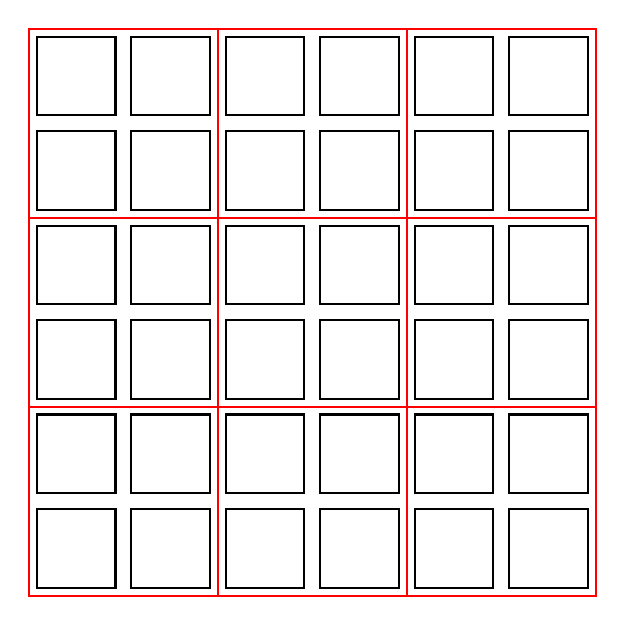
\begin{tikzpicture}
    \tikzstyle{case}=[draw, minimum height=1cm, minimum width=1cm, thick, fill=white, anchor=south west];
    \tikzstyle{redcase}=[draw, minimum height=2.4cm, minimum width=2.4cm, thick, fill=none, draw=red, anchor=south west];

    \foreach \x in {0,...,5} {
        \foreach \y in {0,...,5} {
            \node[case] at (1.2*\y,1.2*\x) {};
        }
    }
    \foreach \x in {0,...,2} {
        \foreach \y in {0,...,2} {
            \node[redcase] at (2.4*\y-0.1,2.4*\x-0.1) {};
        }
    }
\end{tikzpicture}
\end{center}
\end{figure}


The general case can be treated in a similar fashion.

\end{question}

%#############################################################################################################%



%#############################################################################################################%
%#############################################################################################################%
%#############################################################################################################%

\end{document}
